\section{RRT}

The \rrtfunnel\ algorithm will be based upon the general \ac{RRT}
algorithm\cite[LaValle]{article}. This means that it will be sampling based,
picking points uniformly from the state space, an expanding as quickly as it can
into the state-space. An \ac{RRT} algorithm is inherently biased to grow towards
unexplored parts of the state space. A nice way of thinking about the \ac{RRT}
algorithm is as a \textit{Monte-Carlo} method that is biased towards the largest
\textit{Voronoi} of a graph in the configuration space, as shown
in~\ref{subsec:voronoi regions}. 

\subsection{The RRT algorithm}

The \ac{RRT} algorithm is a tree based algorithm which grows a tree in the
configuration space of the robot, starting at the base configuration of the
robot at hand. In order to expand the tree it draws a sample at random from the
configuration space, then tries to connect the new sample with the nearest node
in the tree. Nearest in the sense of some predetermined distance metric. If a
connection can be made -- meaning that it is collision free, and satisfies the
constraints of the dynamical model -- then a new state is added to the tree. If
the sampling is uniform, then the tree is known to have the attribute that the
probability of expanding from an existing node in the tree is proportional the
the \textit{Voronoi region} of that node, and as the largest \textit{Voronoi
  regions} belongs to the states on the leaves of the tree, this means that the
tree will quickly expand into unexplored parts of the state space, as can be
seen in~\ref{fig:rrt-expansion}, and~\ref{fig:voronoi-expansion}.

\begin{figure}
  \includegraphics{figures/rrt/rrt-pseudo.tex} % TODO - this takes the here option?
\end{figure}

\begin{figure}
  \label{fig:rrt-expansion}
  \centering
  \begin{subfigure}[b]{0.3\textwidth}
    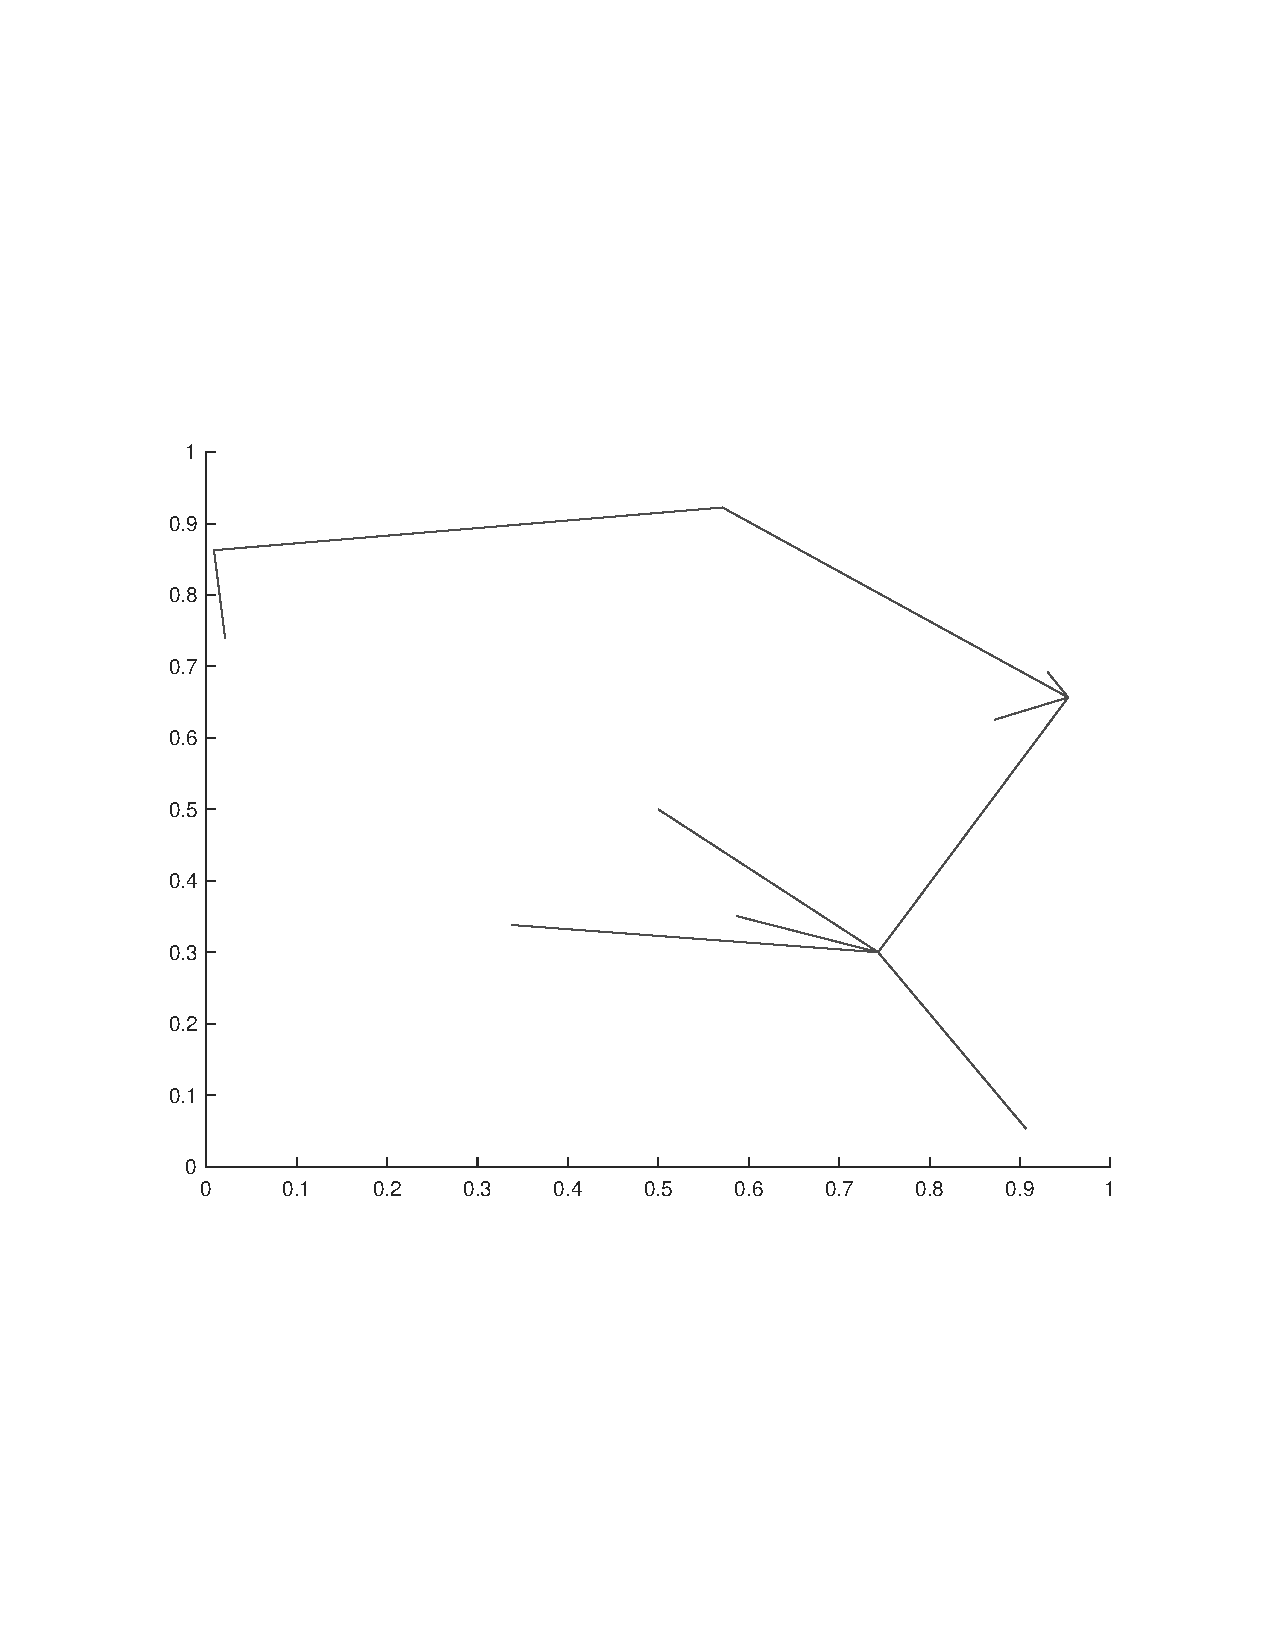
\includegraphics[width=\textwidth]{plainRRT10}
    \caption{RRT-tree after 10 iterations.}
  \end{subfigure}
  \begin{subfigure}[b]{0.3\textwidth}
    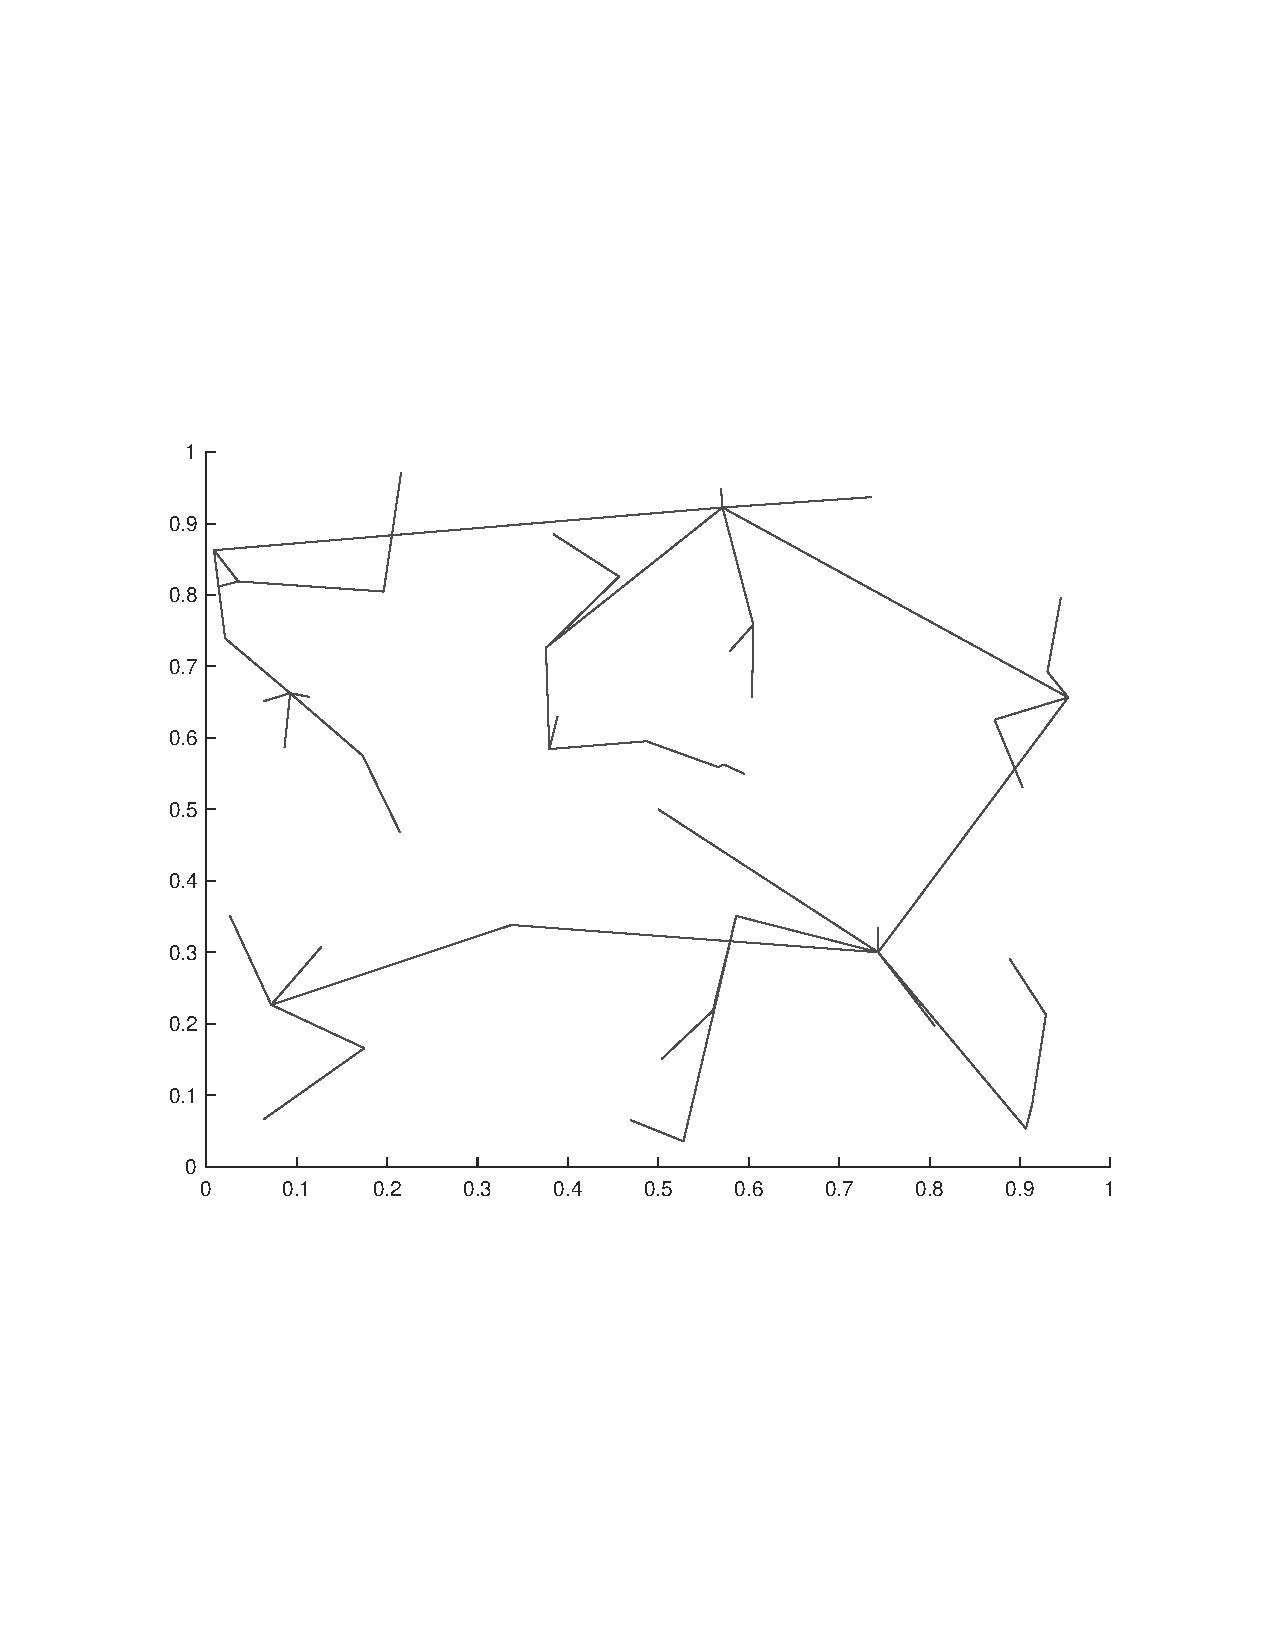
\includegraphics[width=\textwidth]{plainRRT50}
    \caption{RRT-tree after 50 iterations.}
  \end{subfigure}
  \begin{subfigure}[b]{0.3\textwidth}
    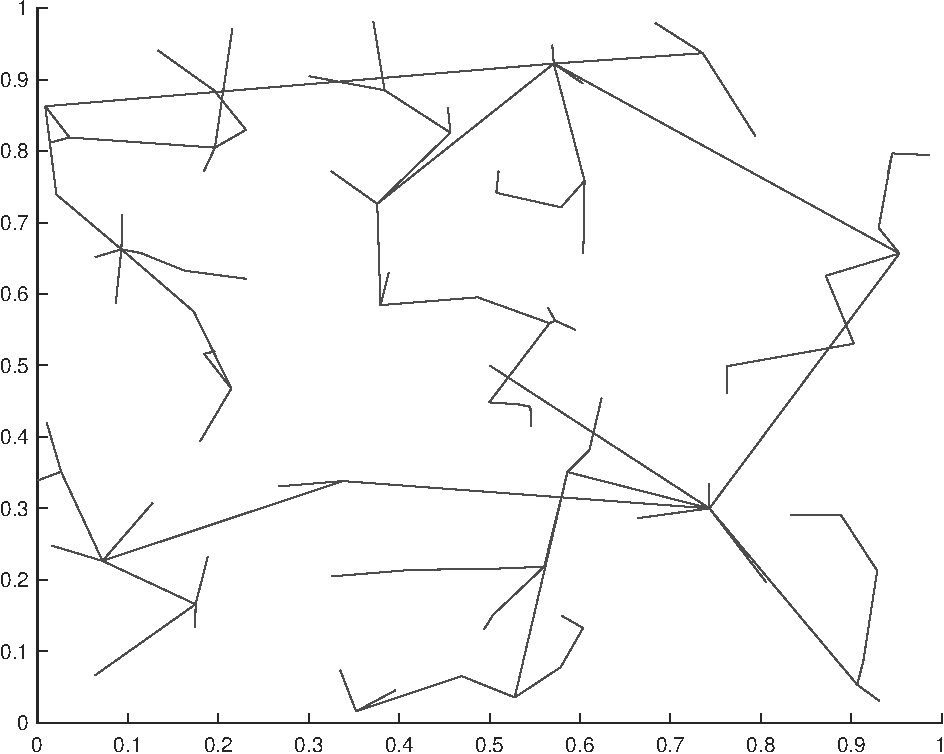
\includegraphics[width=\textwidth]{plainRRT100}
    \caption{RRT-tree after 100 iterations.}
  \end{subfigure}
  \newline % Start the new line of plainRRT10.
  \begin{subfigure}[b]{0.3\textwidth}
    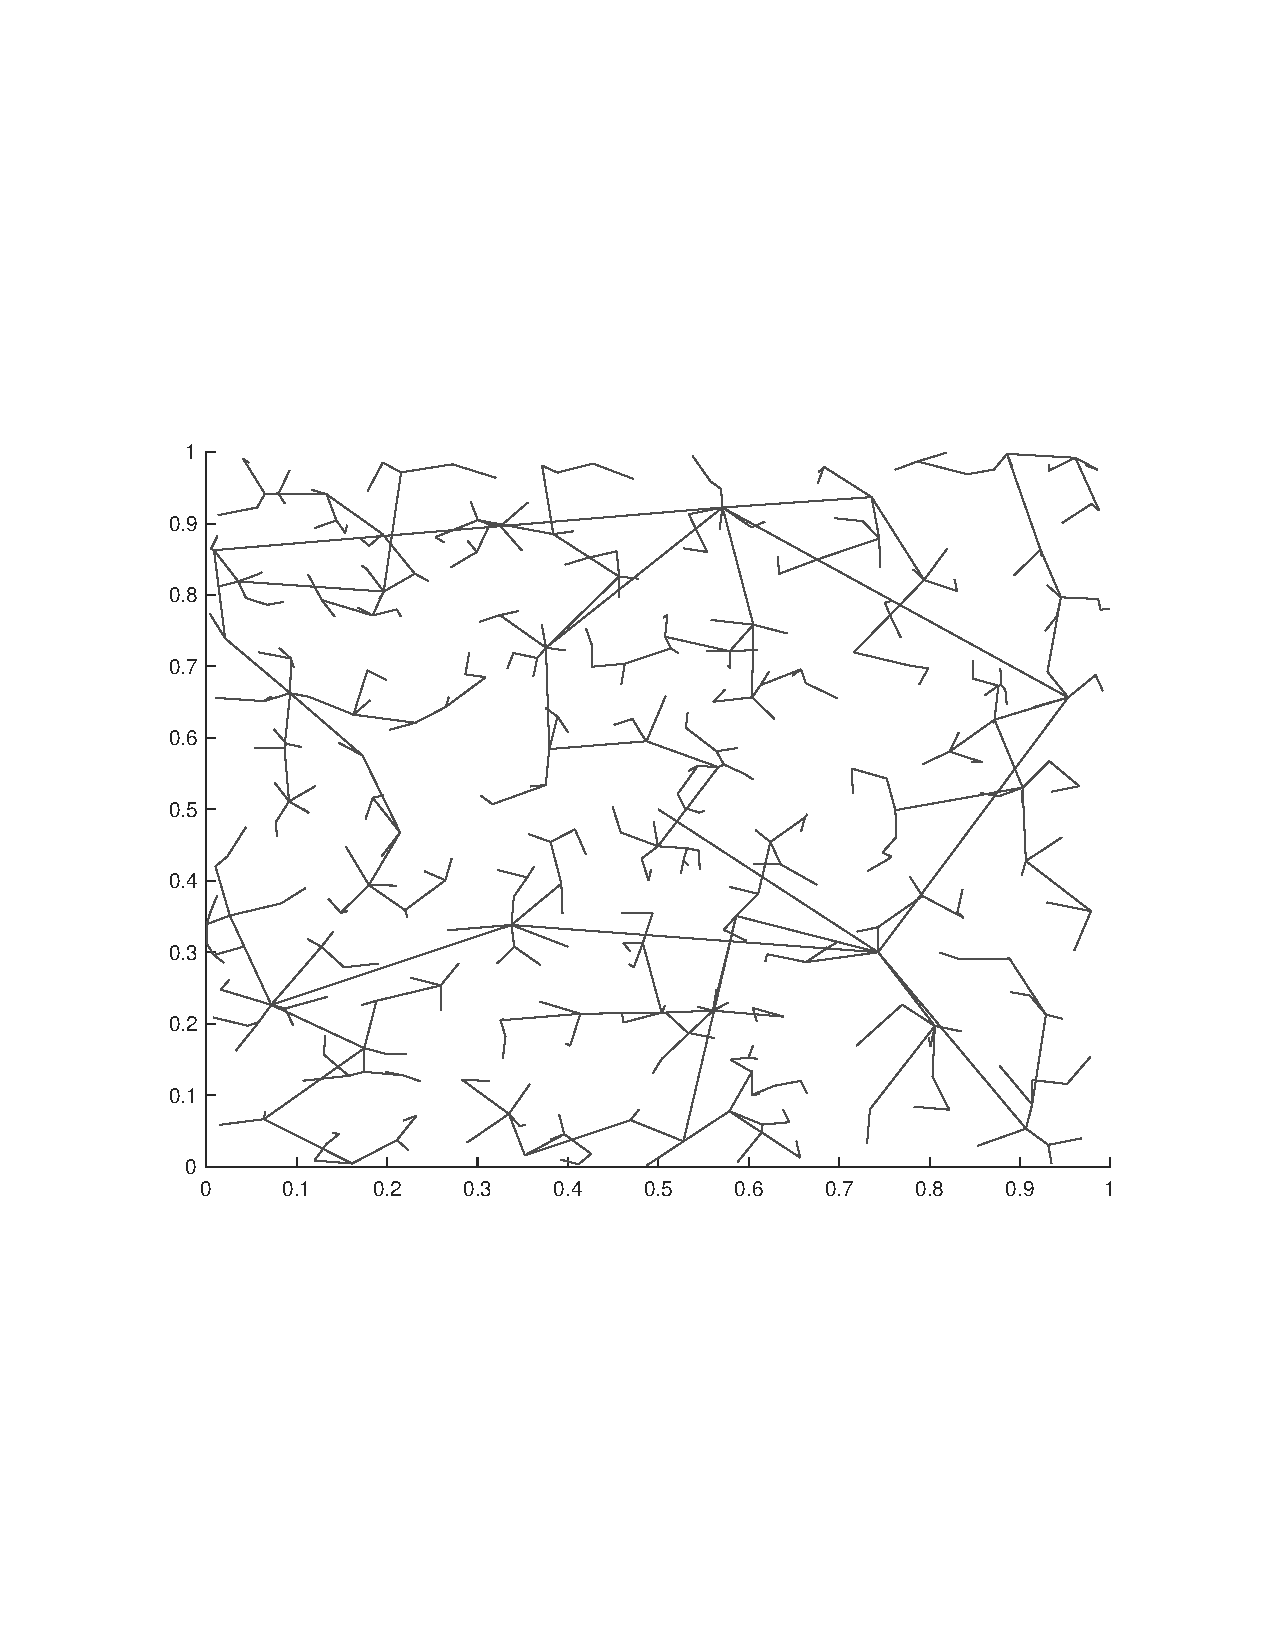
\includegraphics[width=\textwidth]{plainRRT500}
    \caption{RRT-tree after 500 iterations.}
  \end{subfigure}
  \begin{subfigure}[b]{0.3\textwidth}
    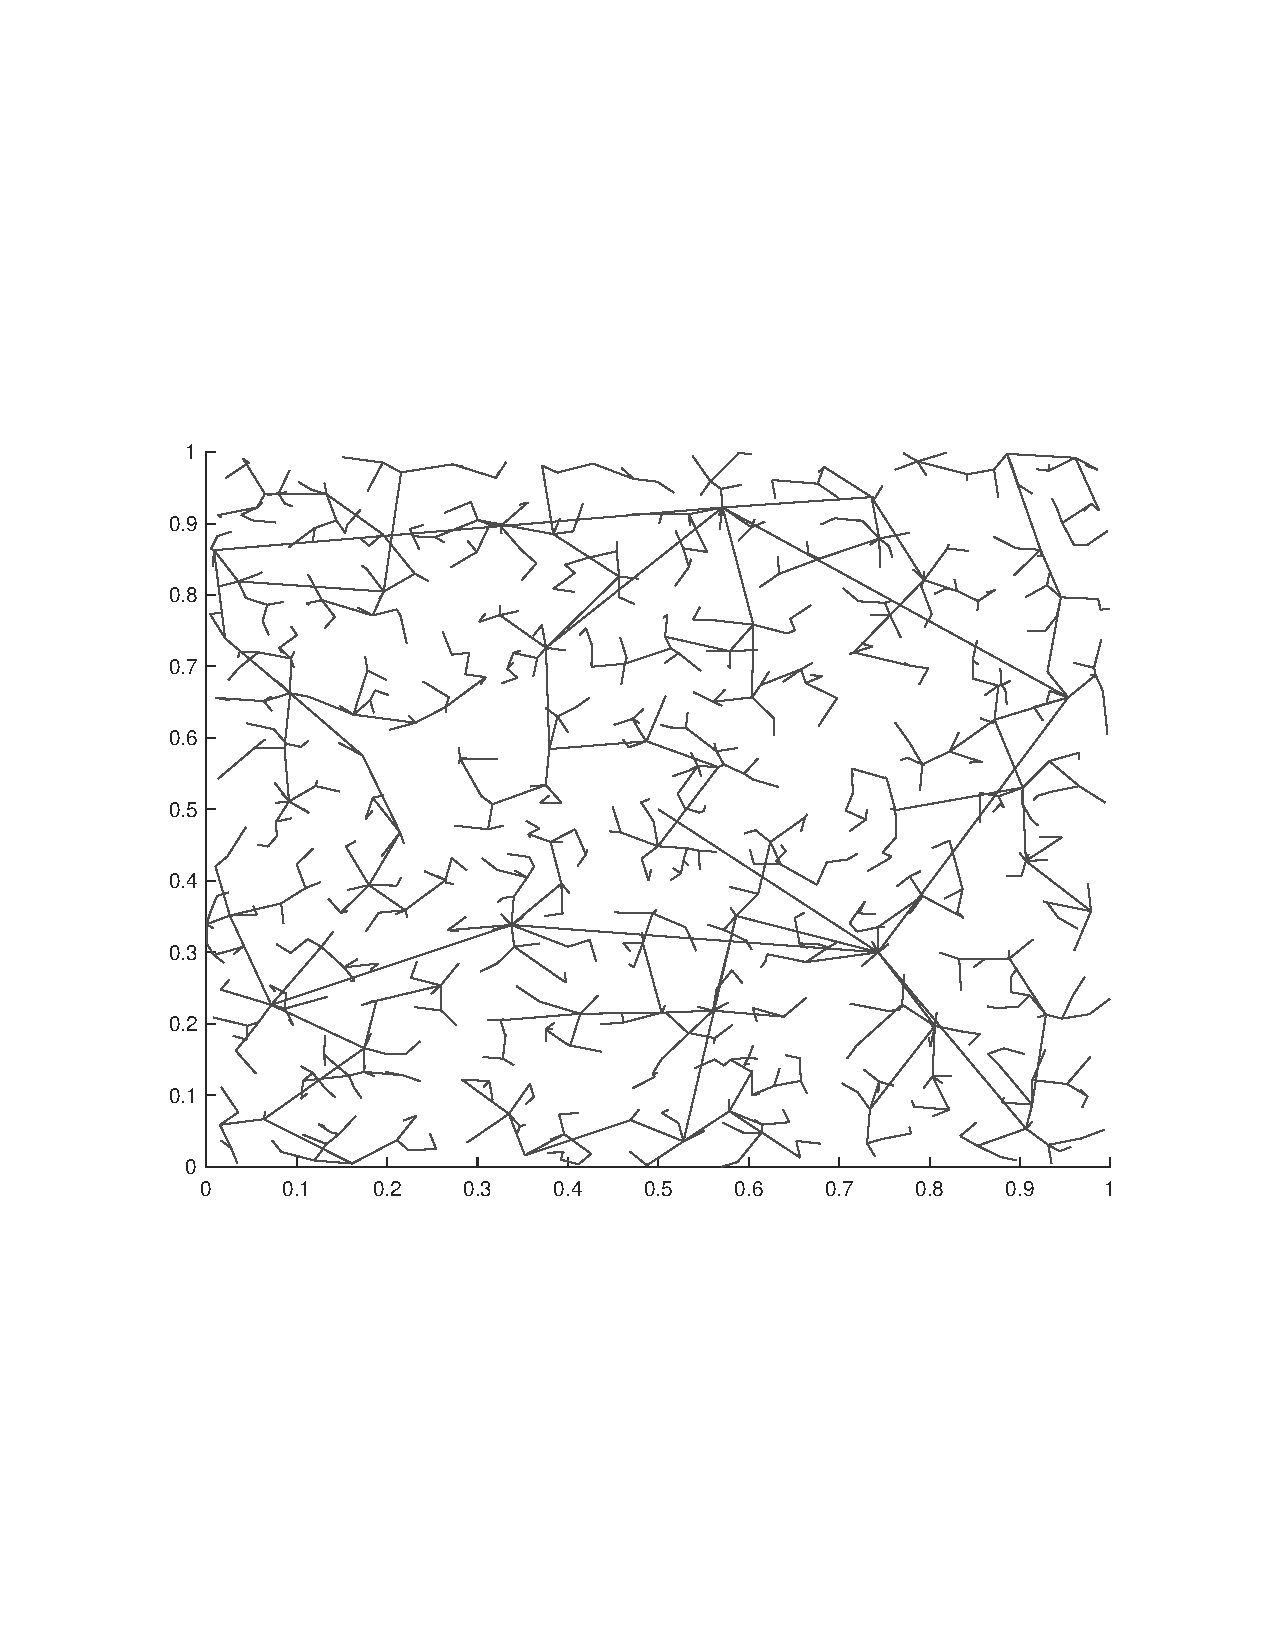
\includegraphics[width=\textwidth]{plainRRT1000}
    \caption{RRT-tree after 1000 iterations.}
  \end{subfigure}
  \begin{subfigure}[b]{0.3\textwidth}
    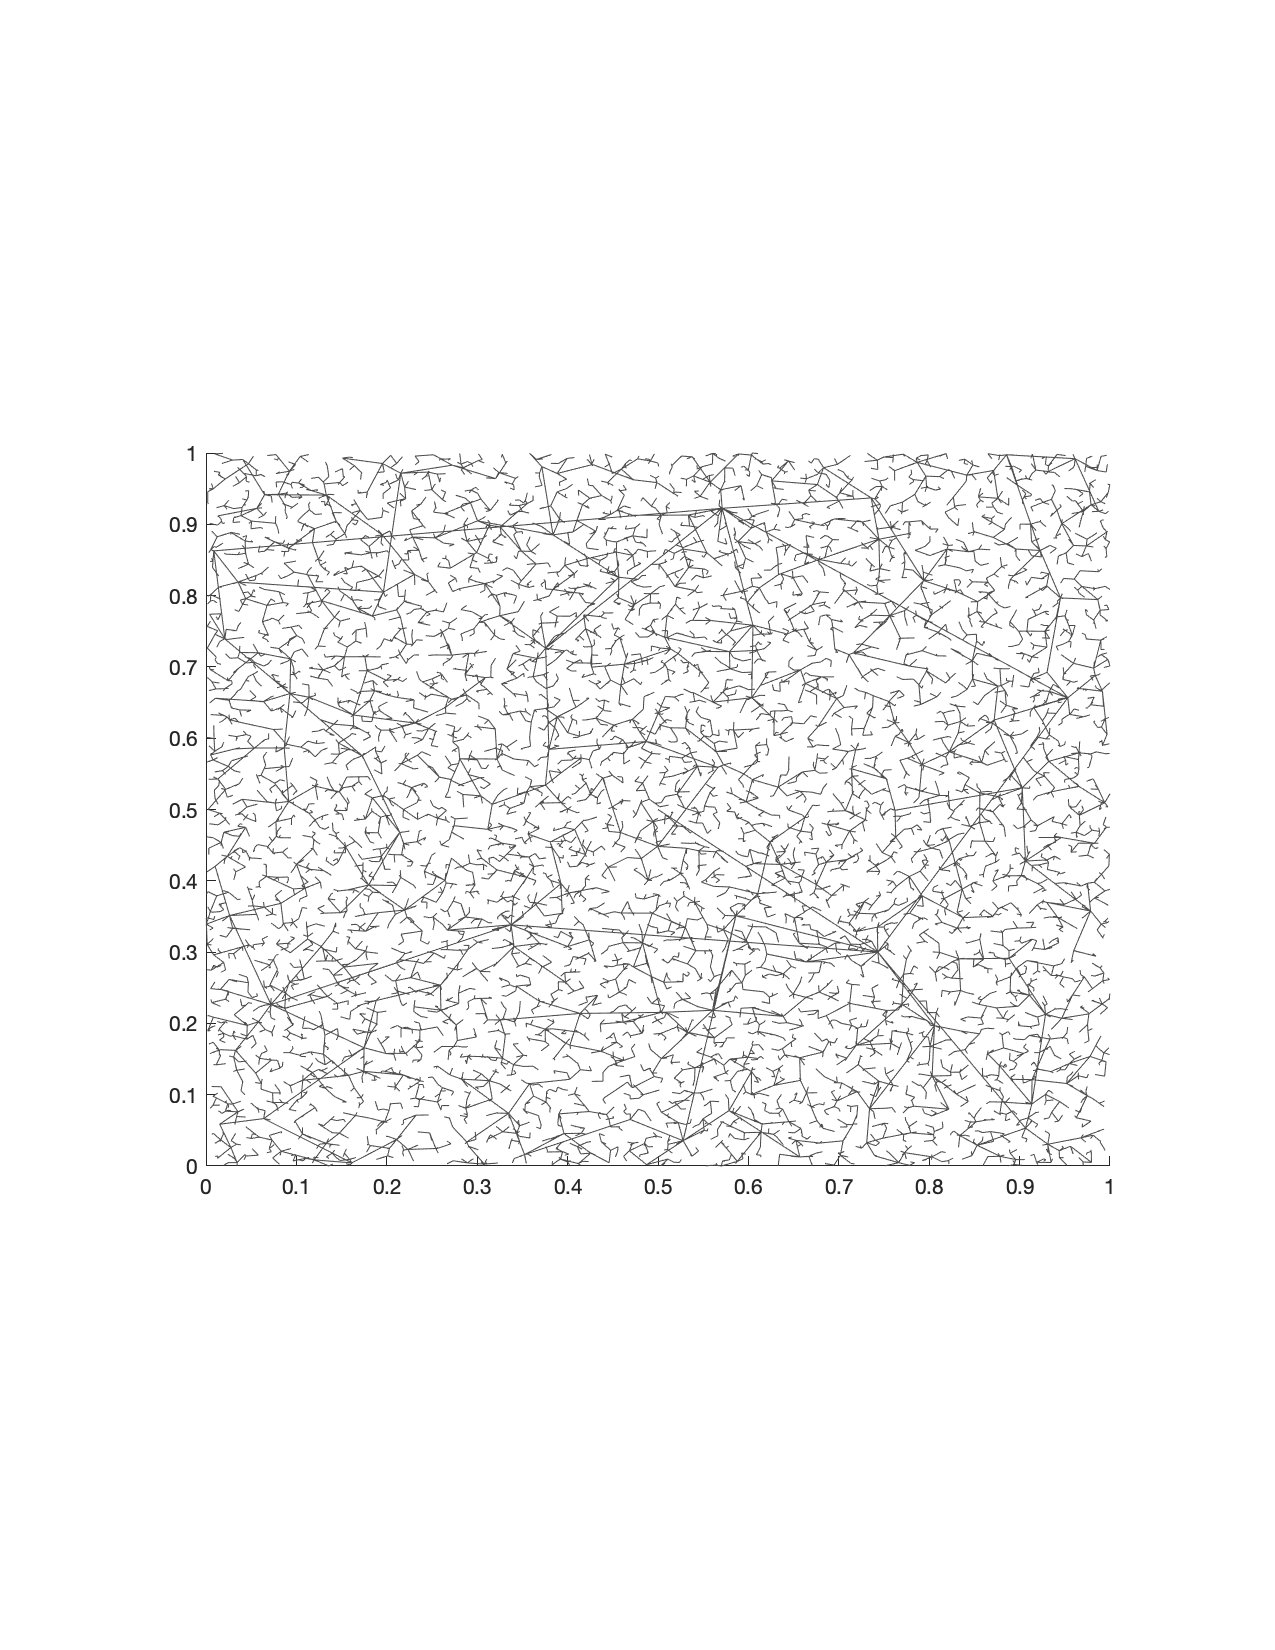
\includegraphics[width=\textwidth]{plainRRT10000}
    \caption{RRT-tree after 10000 iterations.}
  \end{subfigure}
\end{figure}

\subsection{Voronoi diagrams}
\label{subsec:voronoi regions}

Given a number of points in the plane, their Voronoi diagram divides the plane
according the the \textit{nearest neighbour rule}: Each point is associated with
the region of the plane closest to
it~\cite{aurenhammerVoronoiDiagramsSurvey1991}, as can be seen in the
figure~\ref{fig:voronoi-diagram}.

\begin{figure}
  \label{fig:voronoi-diagram}
  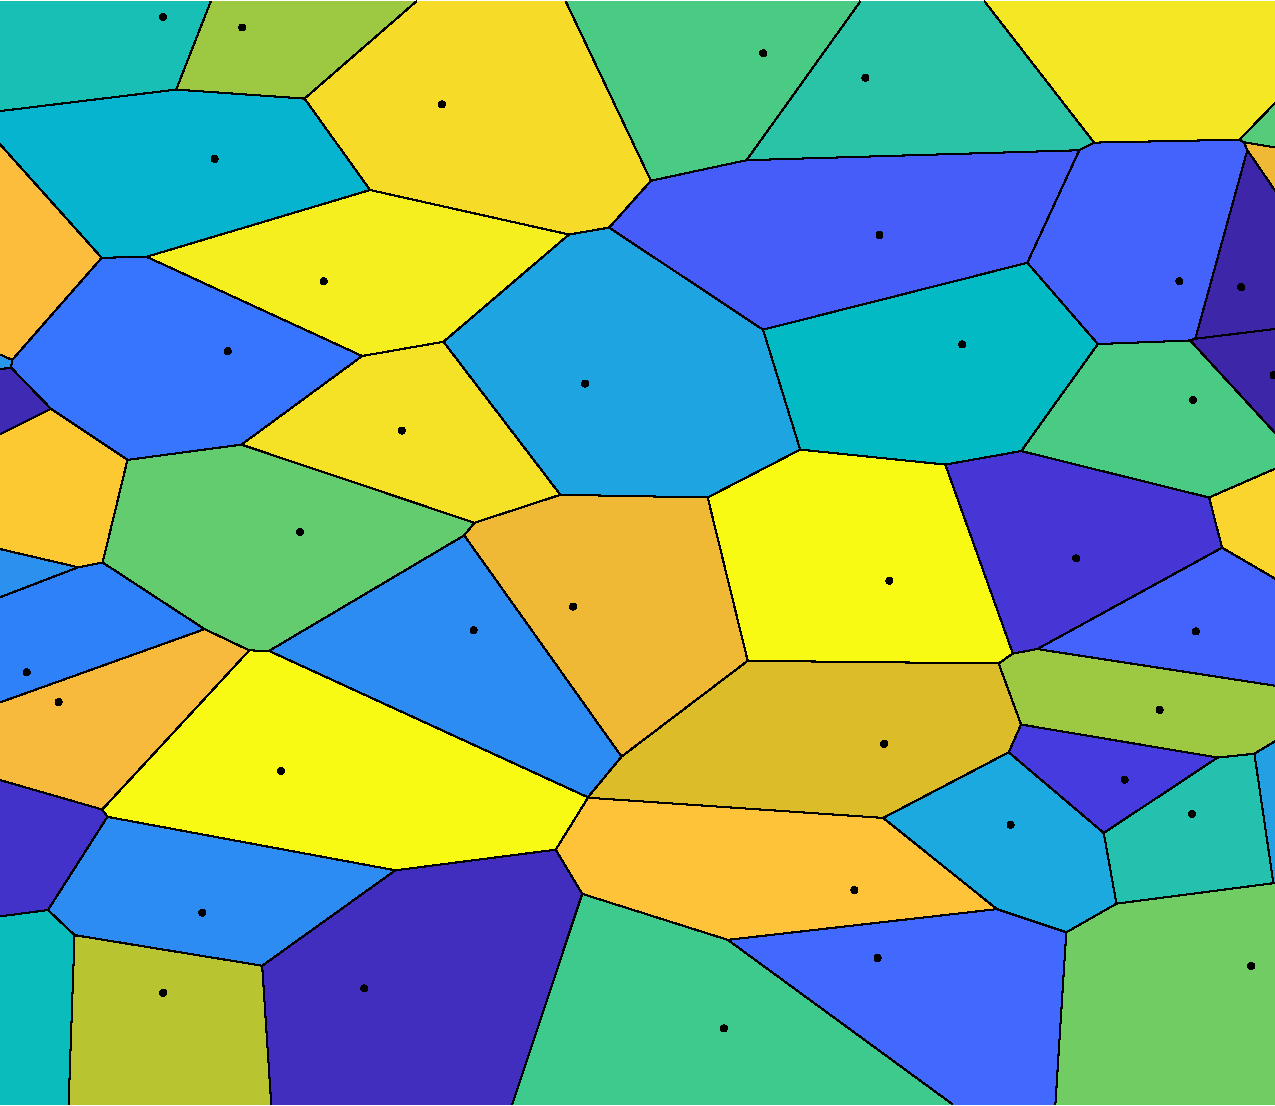
\includegraphics[scale=.3]{figures/rrt/voronoi-diagram}
  \caption{Pictured: The Voronoi regions for a collection of points in the plane,
    using the standard Euclidean metric.}
\end{figure}

When inspecting the Voronoi regions of a \ac{RRT} tree, it is appareant that the
leaf nodes will have the largest Voronoi regions, and thus also the largest
probability for getting expanded, as can be seen in figure~\ref{fig:rrt-voronoi}.

\begin{figure}
  \label{fig:rrt-voronoi}
  \frame{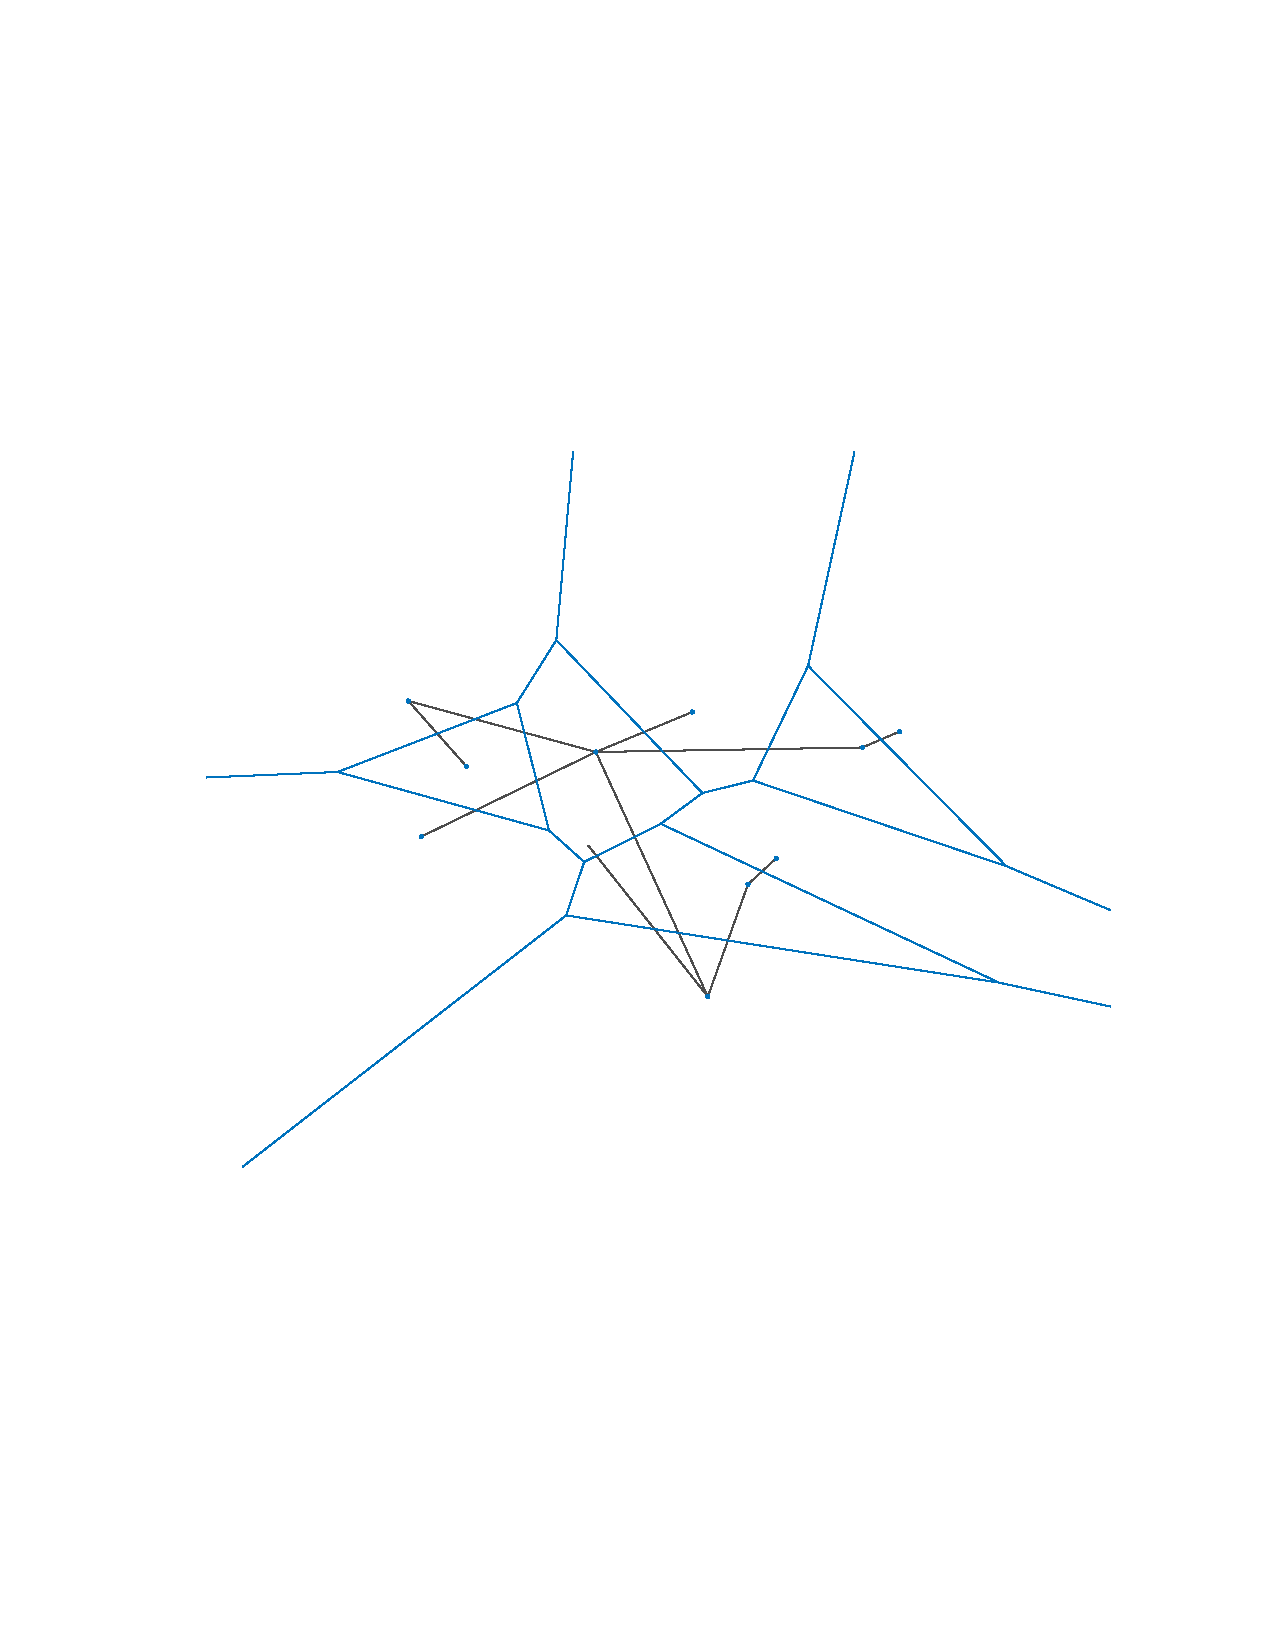
\includegraphics[clip, trim=5cm 9cm 5cm 9cm, scale=.5]{figures/rrt/rrtvoronoi}}
  \caption{Pictured: The voronoi regions for each node in a simple RRT tree,
    which shows how the voronoi bias will lead the algorithm towards unexplored
    areas quickly.}
\end{figure}

\subsection{BiDirectional}
\subsection{Dynamic RRT's?}

\begin{figure}
  \documentclass{standalone}
\usepackage{tikz}

\begin{document}
    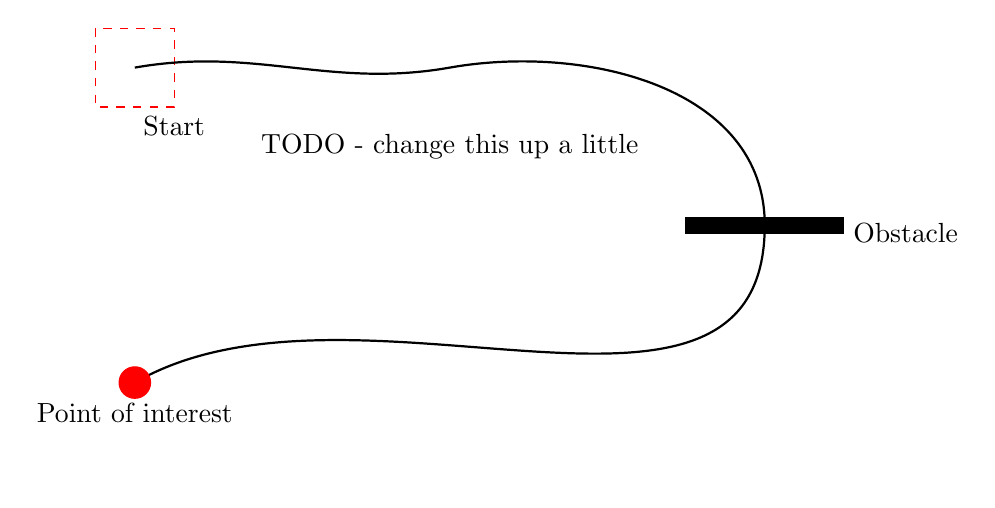
\begin{tikzpicture}
      \draw [red,dashed] (-2.5,2.5) rectangle (-1.5,1.5) node [black,below] {Start}; % Draws a rectangle
      \draw [thick] (-2,2) % Draws a line
      to [out=10,in=190] (2,2)
      to [out=10,in=90] (6,0) 
      to [out=-90,in=30] (-2,-2);    
      \draw [fill] (5,0.1) rectangle (7,-0.1) node [black,right] {Obstacle}; % Draws another rectangle
      \draw [red,fill] (-2,-2) circle [radius=0.2] node [black,below=4] {Point of interest}; % Draws a circle
      \draw node at (2,1) {TODO - change this up a little};
    \end{tikzpicture}
\end{document}
\end{figure}

\subsection{General framework under differential constraints} (LaValle p.676.)


\subsection{RDT}


\subsection{Dynamic RRT}

\subsection{Funnel}

A Funnel is a motion primitive that is `guaranteed' to take the vehicle from a
set of initial conditions to a set of goal states. 

\subsubsection{Composition of funnels}

In essence the 
Each funnel solves the subgoal of getting from the initial set of the funnel to
the goal set. Thus in essence each funnel solves the subproblem of getting from
one funnel to the next, and therefore composing funnels from some global initial
state to the goal state will have solve the motion planning problem with the
guarantees given by the tubes used for the planning task at hand.

TODO - insert pretty picture of funnel with the integral curves of the extremal
paths embedded in beautiful red.

\subsubsection{Reachability plot for the Ground-Vehicle}
TODO - plot the reachability for the ground-vehicle in some time interval using
simulations. 

TODO - plot A reachability tree in 3D using funnels - because different theta's
can exists at the same x,y positiions.

\subsection{Sampling}
It is important that the sampling sequence is dense in the space where sampling
occurs (state-space?), as we want resolution completeness in the end.
\subsubsection{How to obtain uniform sampling}
\subsubsection{How to define a good distance metric}
In general, it is not possible to get a perfect distance metric for our planning
problem, as this involves solving another optimal planning problem, and will
therefore be as, or more complex than the motion planning problem which is
already being solved. Therefore in general we will have to limit ourselves to
approximate distance metrics. The idea is to get as close to the optimal
cost-to-go function without having to compute expensive computations~\cite{LaValle09}.
Distance metrics candidates in the RRT-Funnel algorithm:
\begin{itemize}
  \item Time - Since time can be found by simple summing up the time of all the
    funnels which need be added to get to the certain point in the configuration space.
  \item Lyapunov function - As the Lyapunov function can be seen as an energy
    function, the cost to go to a point can (probably) be used as a metric in
    the planning.
  \item Length of the shortest path between two configurations - ignoring collisions.
  \item A* search heuristics.
  \item Geometric - Stacking Funnels, where the shortest funnel of funnels wins.
    e.g. if the point is not in the cone projected out from the current state by
    the current motion primitives, pick the most extreme turn, and start over
    once again. If it can be reached by a turn, turn, then go straight for N-Funnels.
\end{itemize}

Note that most of these metrics are not metrics in the full sense, as they do
not fulfill the symmetric property, as under dynamic constraints going from a to
b, may not be the same as going from b to a. In most cases it is not true for a
nonholonomic vehicle.

\subsubsection{How to extend the tree?}

Should it be expanded into the dynamic Voronoi regions? If so, what are these regions?


\subsection{Motion Primitives}

A motion primitive is a discrete action chosen from some action set
\(\modelactionspace{}\), and applied as a constant action over a fixed period of
time. The time periods can vary in length, as the primitives do not need to have
the same time length. Thus in the model:

\begin{math}
  x_{k+1} = f_d(x_k,u_k)
\end{math} 

Where \(x_k = x((k-1)\delta{}t)\), and \(u_k\) is the action in
\(\modelactionspace{}_d\) that is applied from time \((k-1)\delta{}t\) to
\(k\delta{}t\). If we let \(\overline{u}^p\) be a motion primitive in
\(\modelactionspace{}\), which is a function from an interval of time, unto
\(modelactionspace{}\). Then by letting the interval of time start at 0 and stop
at \(t_F(\overline{u}^p)\), which has a final time that depends on the
particular prmitive~\cite{LaValle09}.


\subsection{Reachability Graph}

\subsection{RRT-Funnels}


\subsubsection{Transforming and composing the tubes}

If we look at the cyclic coordinates of our model, we can see that using `cyclic
coordinates', the dynamics is independent of position. Or rather:

\begin{math}
  \dot{\dot{q}} = \mathcal{L}(\dot{q},q)
\end{math}

TODO - finish this.


\subsubsection{Using Funnels as motion-primitives}

\subsubsection{Designing good motion primitives}